%%%% ijcai23.tex

\typeout{IJCAI--23 Instructions for Authors}

% These are the instructions for authors for IJCAI-23.

\documentclass{article}
\pdfpagewidth=8.5in
\pdfpageheight=11in

% The file ijcai23.sty is a copy from ijcai22.sty
% The file ijcai22.sty is NOT the same as previous years'
\usepackage{ijcai23}

% Use the postscript times font!
\usepackage{times}
\usepackage{soul}
\usepackage{url}
\usepackage[hidelinks]{hyperref}
\usepackage[utf8]{inputenc}
\usepackage[small]{caption}
\usepackage{graphicx}
\usepackage{amsmath}
\usepackage{amsthm}
\usepackage{booktabs}
\usepackage{algorithm}
\usepackage{amsfonts}
% \usepackage{algorithmic}
\usepackage{algpseudocode}
\usepackage[switch]{lineno}
\usepackage{multirow}
\usepackage{subfigure}

% Comment out this line in the camera-ready submission
\linenumbers

\urlstyle{same}

% the following package is optional:
%\usepackage{latexsym}

% See https://www.overleaf.com/learn/latex/theorems_and_proofs
% for a nice explanation of how to define new theorems, but keep
% in mind that the amsthm package is already included in this
% template and that you must *not* alter the styling.
\newtheorem{example}{Example}
\newtheorem{theorem}{Theorem}

% Following comment is from ijcai97-submit.tex:
% The preparation of these files was supported by Schlumberger Palo Alto
% Research, AT\&T Bell Laboratories, and Morgan Kaufmann Publishers.
% Shirley Jowell, of Morgan Kaufmann Publishers, and Peter F.
% Patel-Schneider, of AT\&T Bell Laboratories collaborated on their
% preparation.

% These instructions can be modified and used in other conferences as long
% as credit to the authors and supporting agencies is retained, this notice
% is not changed, and further modification or reuse is not restricted.
% Neither Shirley Jowell nor Peter F. Patel-Schneider can be listed as
% contacts for providing assistance without their prior permission.

% To use for other conferences, change references to files and the
% conference appropriate and use other authors, contacts, publishers, and
% organizations.
% Also change the deadline and address for returning papers and the length and
% page charge instructions.
% Put where the files are available in the appropriate places.


% PDF Info Is REQUIRED.
% Please **do not** include Title and Author information
\pdfinfo{
/TemplateVersion (IJCAI.2023.0)
}

\title{Relation-specific Entropy-based Knowledge Graph Ensemble}


% Single author syntax
% \author{
%     Hwawoo Jeon^{1,2}, Yoonseob Lim^{1} and Yong Suk Choi^{2}
%     \affiliations
%     Affiliation
%     \emails
%     email@example.com
% }

% Multiple author syntax (remove the single-author syntax above and the \iffalse ... \fi here)
% \iffalse
\author{
Hwawoo Jeon$^{1,2}$\and
Yoonseob Lim$^{1,3}$\And
Yong Suk Choi$^2$
\affiliations
$^1$Center for Intelligent \& Interactive Robotics\unskip,
Korea Institute of Science and Technology\unskip, 136-791\unskip, Seoul\unskip, Korea\\
$^2$The Division of Computer Science and Engineering\unskip,
Hanyang University\unskip, 04763\unskip, Seoul\unskip, Korea\\
$^3$Department of HY-KIST Bio-convergence\unskip,
Hanyang University\unskip, 04763\unskip, Seoul\unskip, Korea\\
\emails
\{feelgood88, yslim\}@kist.re.kr,
cys@hanyang.ac.kr
}
% \fi

\begin{document}

\maketitle

\begin{abstract}
    Knowledge Graph Embedding (KGE) aims to represent entities and relationships from knowledge graphs (KGs) in vector spaces. Existing KGE methods often focus narrowly on specific patterns, which constrains their inferential capabilities to predict diverse relationship patterns. In response to this limitation, we introduce TransEE, a relation-specific entropy-based KG ensemble approach. We assume that the entropy of feature vector similarity is a reliable indicator of the inference potential for particular relations. Following this hypothesis, TransEE utilizes relation-specific ensemble weights, determined by the entropy of feature vector similarity derived from the base model and training data. Moreover, the algorithm is designed to be flexible in adopting base-model combinations, entropy measurement methods, and normalization methods with the goal of effectively applying to various KG data sets and complex prediction environments. Our experiments on the FB15K and FB15k237 datasets, using base models, TransE, TransH, TransR, and TransD, show that TransEE surpasses both single-model and general ensemble methods in prediction accuracy. These results corroborate our hypothesis that the relation-specific entropy of feature vector similarity has correlation with inference performance of KGE.

\end{abstract}

\section{Introduction}

Embedding models may exhibit varying strengths in modeling different types of relation

\section{Related Work}

\subsection{Knowledge Graph Embedding}

Translation-Based Embedding algorithms use very little parameters to model the multi-relational data but outperform traditional sophisticated methods. The score functions of Translation-Based Embedding algorithms are defined as the following Table ~\ref{tab:score}. 

TransE~\cite{bordes2013translating} model is the earliest proposed Translation-Based Embedding algorithm in 2013, which takes the relations as the translating operations from these head entities to tail entities on a continuous low-dimensional vector space. It only performs well for modeling the 1-to-1 semantic relations. Where \(\textbf{h}\) represents the embedding of the head entity, \(\textbf{r}\) represents the embedding of the relation, \(\textbf{t}\) represents the embedding of the tail entity. TransH~\cite{wang2014knowledge} model projects head and tail entities vectors into the hyper-planes of the relations where completing the translating operations. TransH~\cite{wang2014knowledge} model significantly improves TransE~\cite{bordes2013translating} model on N-to-1 and N-to-N types of semantic relations. Where \(\textbf{w}_r\) represents the hyperplane normal vector for relation \(\textbf{r}\). TransR~\cite{lin2015learning} is another extension of TransE~\cite{bordes2013translating} that considers relation-specific projection matrices. It allows entities and relations to exist in different vector spaces, and mappings are learned to project entities into relation-specific spaces. Where \(\textbf{M}_r\) represents the projection matrix for relation \(r\). TransD~\cite{ji2015knowledge} is an improved version of TransR~\cite{lin2015learning} that addresses the overfitting issue by introducing relation-specific translation matrices. It allows for flexible modeling of relations. Where \(\textbf{M}_r\) represents the relation-specific translation matrix.

\subsection{Knowledge Graph Ensemble}

\begin{table}[!tb]
    \centering
    \begin{tabular}{ll}
        \hline
        Model  & Score Function \\
        \hline
        TransE  & $s^{TransE}(h, r, t) = ||h + r - t||_2$\\
        TransH  & $s^{TransH}(h, r, t) = ||h + r - t - \textbf{w}_r(\textbf{w}_r^\top(h - t))||_2$\\
        TransR  & $s^{TransR}(h, r, t) = ||\textbf{M}_r h + r - \textbf{M}_r t||_2$\\
        TransD  & $s^{TransD}(h, r, t) = ||\textbf{M}_r (h + r) - \textbf{M}_r (t + r)||_2$\\
        \hline
    \end{tabular}
    \caption{Score functions of translation based embedding models}
    \label{tab:score}
    
\end{table}



data data data data data data data data data data data data data data data data data data data data data data data data data data data data data data data data data data data data data data data data data data data data data data data data data data data data data data data data data data data data data data data data data data data data data data data data data data data data data data data data data data data data data data data data data data data data data data data data data data data data data data data data data data data data data data 
\section{Method}

\bgroup
\begin{figure*}[t]
  \centering \makeatletter\IfFileExists{Images/Figure1.png}{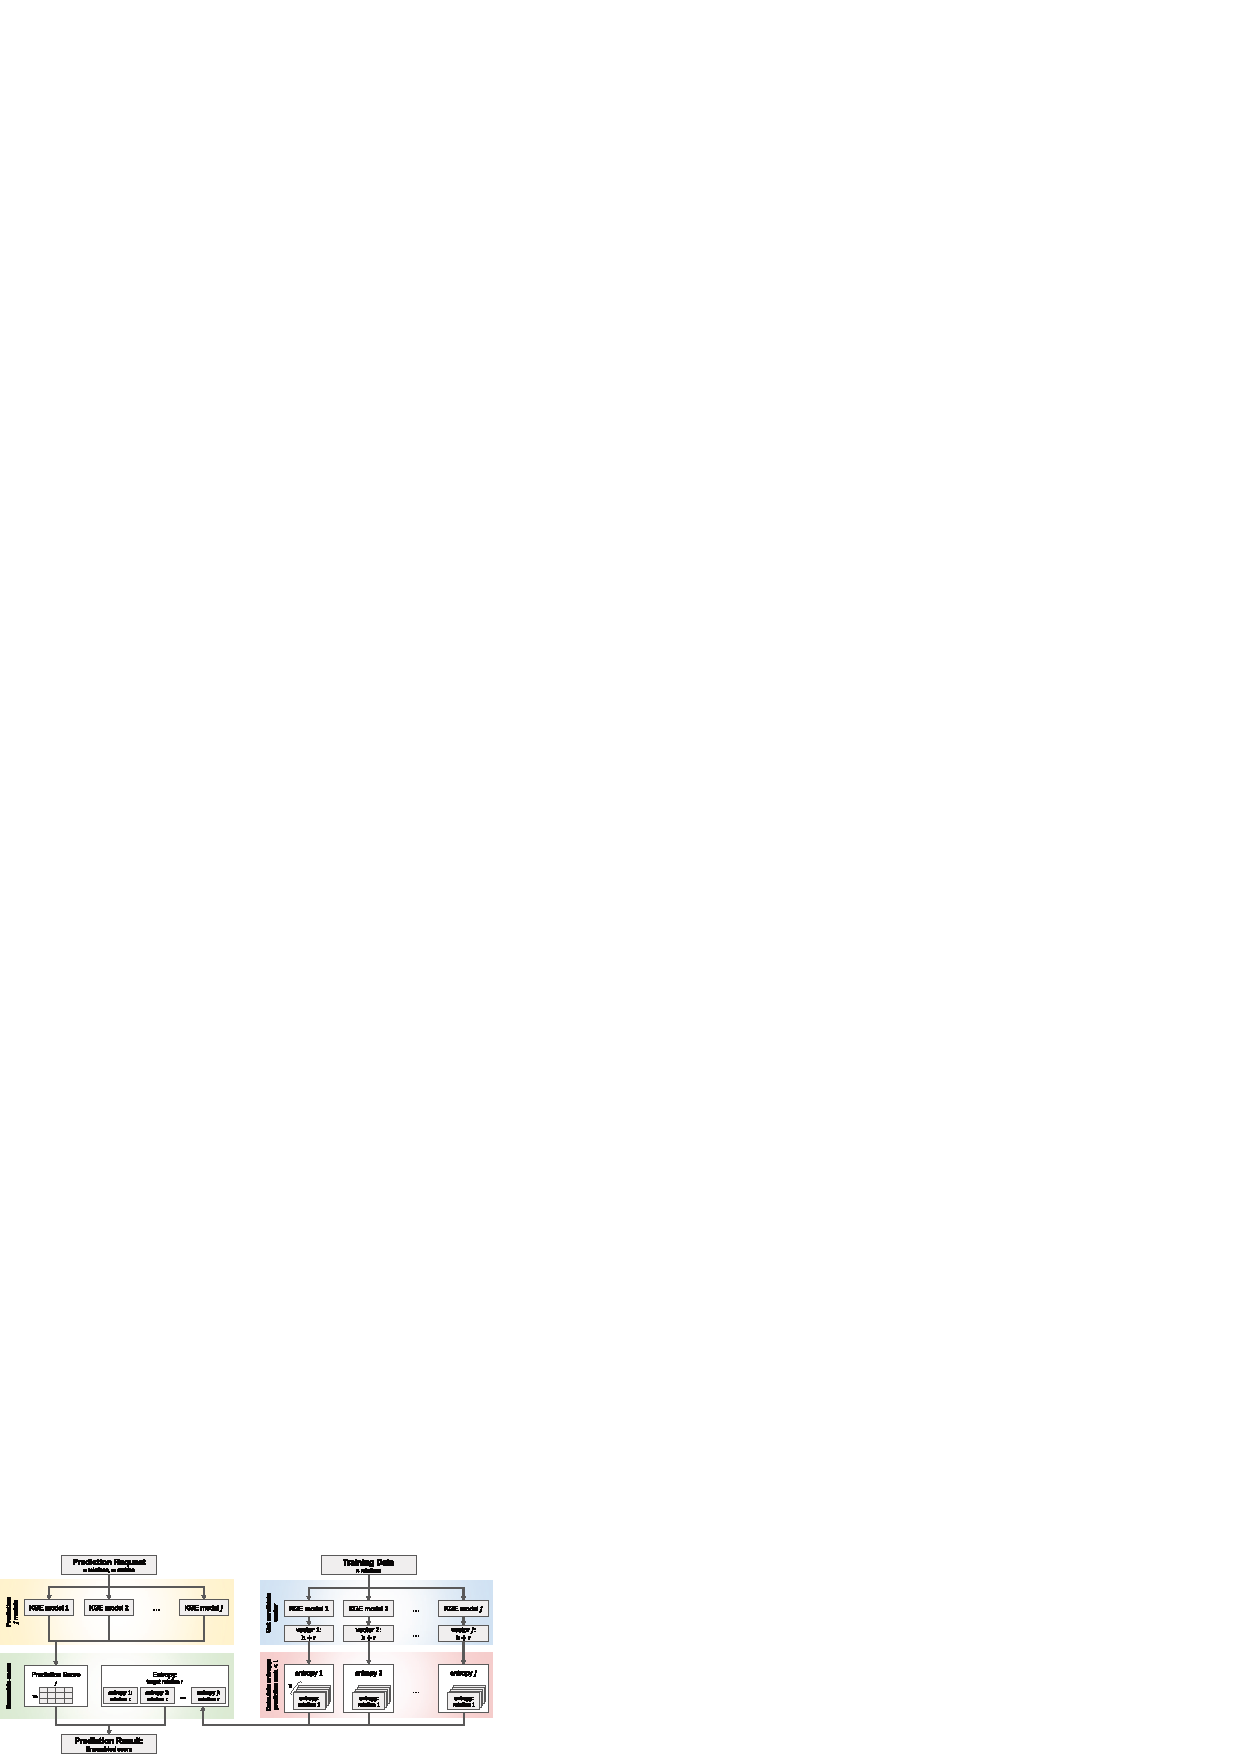
\includegraphics[width =0.65\textwidth]{Images/Figure1.png}}{}
  \makeatother
  \caption{{System Architecture.}}
  \label{fig:sysArch}
  \hfill
\end{figure*}
\egroup


In this section, we introduce a approach for calculating the relation-specific entropy weight in the context of link prediction in knowledge graphs. Our method leverages various embedding models to predict the likelihood of a relationship between two entities. The overview of our approach is outlined in Figure~\ref{fig:sysArch}. Additionally, The core of our method is the entropy weight calculation algorithm, which we present in Algorithm \ref{alg:linkPredictOverview}. 


The ensemble method combines the predictive capabilities of each base model, accounting for their individual uncertainties in prediction, to yield a more robust and reliable prediction score. 






The algorithm largely consists of an ensemble-based link prediction component and a relation-specific entropy calculation component. An ensemble that uses the relation-specific entropy of each model as a weight is presented in Section 1. The calculation of the relation-specific entropy of each base model using the training data set is presented in Section 2. 



% \subsection{Link Prediction Process}



\begin{algorithm}[!htb]
    \caption{Link Prediction: entropy base ensemble}
    \label{alg:linkPredictOverview}
    \textbf{Input}: Request triple $\{(h, r, t) \;:\; h,t \in E, r \in R\}$, base models $\{\mathcal{M}_i \;:\; i \in N\}$, minimum number of vectors $minLen$ for entropy calculation, type of entropy normalization $norm$, type of entropy $\mathit{type}$, type of distance $\mathit{dist}$, minimum hit rank $k$, and min-max range of normalization for base prediction score $\delta^{s}$ and ensemble weight $\delta^{w}$.\\
    \textbf{Parameter}: Prediction score $\{s\acute{}_{i} \;:\; i \in N\}$ of base models $\mathcal{M}$, relation-specific entropy $\{\mathcal{H}^{i} \;:\; i \in N\}$, number of resource size $\{resSize^{i} \;:\; i \in N\}$ which used in entropy calculation, relation-specific ensemble weights $\{\mathcal{W}^i \;:\; i \in N\}$, Training data triple $\tau_{hrt} = \{(h, r, t)\;:\; \tau_{htr} \in T, (h, t) \in E, r \in R \}$, base models $\mathcal{M} = \{m_1, m_2, \ldots, m_N\}$, embedded vector $\mathbf{v}_{hrt}^i = \{(h\acute{}, r\acute{}, t\acute{})\;:\; i \in {N}\}$\\
    \textbf{Output}: Ensemble prediction Score $\mathcal{S}$.\\
    
    \begin{algorithmic}[1] %[1] enables line numbers      
    
        \Statex \hrulefill
        \Statex \noindent\underline{\hbox to \linewidth{\textbf{Link-prediction sequence}\hfill}}
        \Statex Calculate base prediction score $s\acute{}$
        \State $s\acute{}_i \leftarrow \{Norm_{\text{minmax}}(s^i(h, r, t), \delta^{S}) \;|\; \forall i \in N\}$
        
        \Statex
    
        \Statex Determine ensemble weight $\mathcal{H}$ and their number of resource vector $resSize$.
        \vspace{3pt}
        \State $\mathcal{H}, resSize \leftarrow \Call{EntropyWeight}{\mathcal{M}, r}$
        \Statex

        \Statex Ensemble for final prediction score $\mathcal{S}$.
        \vspace{3pt}
        \State $\mathcal{W}^i \leftarrow \{Norm_{norm}(\mathcal{H}^i, \delta^{W}) \;|\; resSize^{i}>minLen\}$
        \vspace{3pt}

        \If{$\Call{Len}{\mathcal{W}} < 1$}
            \vspace{3pt}
            \State $\mathcal{W}^i \leftarrow \{1\;|\; \forall i \in N\}$
            \vspace{3pt}
        \EndIf
            
        \vspace{3pt}
        \State $\mathcal{S} \leftarrow \sum_{m=1}^{N} s\acute{}_i \mathcal{W}i$
        \Statex
        \State \Return $\mathcal{S}$
        \Statex \hrulefill
        \Statex \noindent\underline{\hbox to \linewidth{\textbf{Relation-specific entropy calculation}\hfill}}
        \Function{EntropyWeight}{$\mathcal{M}, r, k, type, dist$}

            \State $row \leftarrow \{\tau_{hxt}\;|\; x=r, \forall \tau \in T\}$
        
            \For{$i$ in $N$}
                \vspace{3pt}
                \State $res^{i} \leftarrow \{\mathcal{V}^i(\mathbf{v}_{\tau})\;|\;\mathrm{avg}(rank_{\tau}) <k \}$
                \vspace{3pt}
                \State $prob^{i} \leftarrow Probs(D_{\mathit{dist}}(res^{i}, res^{i}))$
                \vspace{3pt}
                \State $\mathcal{E}^{i} \leftarrow \mathcal{H}^{\mathit{type}}(prob_r^m)$
                \vspace{3pt}
                \State $resSize^{i} \leftarrow \mathtt{len}(res^{i})$  
                \vspace{3pt}
            \EndFor
            \vspace{3pt}
            \State \Return $\mathcal{E}, resSize$
            
        \EndFunction
    \end{algorithmic}
\end{algorithm}


% Relation-specific ensemble can be written as follows:



% \begin{equation}
%     \resizebox{.50\linewidth}{!}{$
%             \begin{gathered}
%                 \mathcal{W} = Norm_{norm}(\mathcal{E}, range), \\            
%                 \mathcal{S} = \sum_{m=1}^{N} s\acute{}_i \mathcal{W}_i
%             \end{gathered}
%         $}
% \end{equation}
% % \begin{equation}
% %     \resizebox{.32\linewidth}{!}{$
% %             \displaystyle
% %             \mathcal{S} = \sum_{m=1}^{N} s\acute{}_i \mathcal{W}_i
% %         $}.
% % \end{equation}



\subsection{Ensemble Weight: Entropy}

In this section, we introduce a approach for calculating the relation-specific entropy weight in the context of link prediction in knowledge graphs. Our method leverages various embedding models to predict the likelihood of a relationship between two entities. The core of our method is the entropy weight calculation algorithm, which we present in Algorithm \ref{alg:entropy}. 

The entropy weight calculation algorithm (see Algorithm \ref{alg:entropy}) computes the entropy weight for a target relation in a knowledge graph. The algorithm takes as input a target relation, the type of entropy, the type of distance measure, a minimum hit rank, and the prediction mode. It operates on a set of training data triples and a collection of base models, producing as output the entropy calculation result and the size of the resource.

\begin{algorithm}[!b]    
    \caption{Entropy Weight Calculation}
    \label{alg:entropy}
    \textbf{Input}: Target relation $r \in R$, type of entropy $\mathit{type}$, type of distance $\mathit{dist}$, minimum hit rank $k$, prediction mode $mode$.\\\\ 
    \textbf{Parameter}: Training data triple $\tau_{hrt} = \{(h, r, t)\;:\; \tau_{htr} \in T, (h, t) \in E, r \in R \}$, base models $\mathcal{M} = \{m_1, m_2, \ldots, m_N\}$, embedded vector $\mathbf{v}_{hrt}^i = \{(h\acute{}, r\acute{}, t\acute{})\;:\; i \in {N}\}$.\\\\
    \textbf{Output}: Entropy calculation result $\mathcal{E}$, number of resource size $resSize$.\\
    \begin{algorithmic}[1] %[1] enables line numbers

        \State $row \leftarrow \{\tau_{hxt}\;|\; x=r, \forall \tau \in T\}$
        
        \For{$i$ in $N$}
            \vspace{3pt}
            \Statex \hspace*{1em} // rank of link-prediction about each model
            % \Statex \hspace*{1em} // $rank = \{rank(h,r,t) \;:\; \forall (h, r, t) \in row\}$
            \State $rank \leftarrow \{\mathtt{Rank}(s^i(\tau)\;|\; \forall \tau \in row\}$
            \vspace{3pt}

            % \If{$mode \text{ is } haed$}
                % \vspace{3pt}
                \State $res^{i} \leftarrow \{\mathcal{V}^i(\mathbf{v}_{\tau})\;|\;\mathrm{avg}(rank_{\tau}) <k \}$     
            %     \vspace{3pt}
            % \Else
                % \vspace{3pt}
                % \State $res_{h}^{i} \leftarrow \{\mathcal{V}^{i}(\mathbf{v}_{row})\;|\;\mathrm{avg}(rank_{h,t\acute{}}) <k \}$     
            %     \vspace{3pt}
            % \EndIf
            % \vspace{3pt}            
            % \State $pdist^{i} \leftarrow D_{\mathit{dist}}(res^{i}, res^{i})$
            \vspace{3pt}
            \State $prob^{i} \leftarrow Probs(D_{\mathit{dist}}(res^{i}, res^{i}))$
            \vspace{3pt}
            \State $\mathcal{E}^{i} \leftarrow \mathcal{H}^{\mathit{type}}(prob_r^m)$
            \vspace{3pt}
            \State $resSize^{i} \leftarrow \mathtt{len}(res^{i})$  
            \vspace{3pt}
        \EndFor
        \vspace{3pt}
        \State \Return $\mathcal{E}, resSize$
    \end{algorithmic}
\end{algorithm}

\vspace{10pt}

The entropy weight calculation algorithm (see Algorithm \ref{alg:entropy}) computes the entropy weight for a target relation in a knowledge graph. The algorithm takes as input a target relation, the type of entropy, the type of distance measure, a minimum hit rank, and the prediction mode. It operates on a set of training data triples and a collection of base models, producing as output the entropy calculation result and the size of the resource.

\subsubsection{Input and Parameters}
The algorithm takes as input a target relation from a set of relations \( R \), along with the type of entropy and distance metrics, a minimum hit rank \( k \), and the prediction mode. The parameters include training data triplets \( \tau_{hrt} \) and base models \( \mathcal{M} \). These inputs and parameters lay the foundation for calculating the entropy weight, a measure crucial for evaluating the performance of KGE models in link prediction tasks.

\subsubsection{Rank Calculation}
For each model \( m \) in \( \mathcal{M} \), the algorithm computes the rank of link prediction for each triplet in the training data using each score functions (See Table~\ref{tab:score}). This step is vital as it establishes a baseline for evaluating how well each model predicts the existence of a link within a given triplet.

\subsubsection{Resource Extraction}
Depending on the prediction mode, the algorithm extracts a set of predicted vectors for relation-specific resources. This is contingent on the average rank and a predefined minimum hit rank \( k \). The extraction process is different for head and tail prediction modes, reflecting the asymmetry often inherent in real-world relational data. The example about TransE~\cite{bordes2013translating} define as:
\begin{equation}
    \resizebox{.91\linewidth}{!}{$
            \displaystyle
            \mathcal{V}^{TransE}(\mathbf{v}_{htr}, mode) = \begin{cases}
                    t\acute{}-r\acute{} & \text{if mode = head} \\
                    h\acute{}+r\acute{} & \text{if mode = tail} \\
                \end{cases}
        $}.
\end{equation}

\subsubsection{Distance Calculation}
After extracting the resources, the algorithm computes pairwise distances such as, either Euclidean or cosine similarity. The choice of distance metric can significantly affect the outcome, as it captures different aspects of similarity or dissimilarity between data points. In this paper, we used Euclidean and cosine similarity, their defines as:
\begin{equation}
    \resizebox{.73\linewidth}{!}{$
            \displaystyle
            D_{\text{euclidean}}(A_i, A_j) = \sqrt{\sum_{k=1}^{m}(A_{ik} - A_{jk})^2}
        $},
\end{equation}
\begin{equation}
    \resizebox{.88\linewidth}{!}{$
            \displaystyle
            D_{\text{cosine}}(A_i, A_j) = 1 - \frac{\sum_{k=1}^{m}A_{ik} \times A_{jk}}{\sqrt{\sum_{k=1}^{m}A_{ik}^2} \times \sqrt{\sum_{k=1}^{m}A_{jk}^2}}
        $}.
\end{equation}

\subsubsection{Probability Density Function}
The algorithm employs a probability distribution to analyze the distances. Empirically, we used Burr~\cite{burr1942cumulative} distribution, defined as:  
\begin{equation}
    \resizebox{.70\linewidth}{!}{$
            \displaystyle
            Probs(x; c, d) = cd \frac{x^{c-1}}{(1 + x^c)^{d+1}}
        $}.
\end{equation} Where \( x \geq 0 \) is a variable, \( c > 0 \) and \( k > 0 \) are shape parameters. In Figure ~\ref{fig:pdfhist}, we present a histogram illustrating pairwise distances and probability density function for the Burr distribution. This figure compares the Euclidean and cosine similarities within the TransD model, focusing on a specific relation from the FB15k237 dataset.


\bgroup
\begin{figure}[!tb]
  \centering \makeatletter\IfFileExists{Images/Figure2.png}{\includegraphics[width =0.48\textwidth]{Images/Figure2.png}}{}
  \makeatother
  \caption{{Compare of probability density function and pairwise distance histogram.}}
  \label{fig:pdfhist}
  \hfill
\end{figure}
\egroup


\subsubsection{Entropy Calculation}
Subsequently, entropy is computed based on the specified type. Entropy here serves as a measure of uncertainty or diversity in model predictions, providing a quantifiable metric to assess the effectiveness of different KGE models. The example of types of entropy equation about Shannon and Rényi as follows:

\begin{equation}
    \label{eq:shannon}
    \resizebox{.68\linewidth}{!}{$
            \displaystyle
            \mathcal{H}^{shannon}(X) = -\sum_{i} p(x_i) \log p(x_i)
        $}.
\end{equation}
\begin{equation}
    \label{eq:renyi}
    \resizebox{.68\linewidth}{!}{$
            \displaystyle
            \mathcal{H}_{\alpha}^{r\acute{e}nyi}(X) = \frac{1}{1-\alpha} \log \left( \sum_{i} p(x_i)^\alpha \right)
        $}.
\end{equation}



% 1. \textbf{Rank Calculation}: For each model in $\mathcal{M}$, the algorithm calculates the rank of link prediction for each triplet in the training data using each score functions (See Table~\ref{tab:score}).


% 2. \textbf{Resource Extraction}: Depending on the prediction mode (head or tail), the algorithm extracts a predict vector set of resources based on the average rank and the predefined minimum hit rank $k$. predicted vector is calculated depending on each models. the example about TransE~\cite{bordes2013translating} define as:
% \begin{equation}
%     \resizebox{.91\linewidth}{!}{$
%             \displaystyle
%             \mathcal{V}^{TransE}(\mathbf{v}_{htr}, mode) = \begin{cases}
%                     t\acute{}-r\acute{} & \text{if mode = head} \\
%                     h\acute{}+r\acute{} & \text{if mode = tail} \\
%                 \end{cases}
%         $}.
% \end{equation}


% 3. \textbf{Distance Calculation}: The pairwise distance is computed using either the Euclidean or cosine metric defines as: 
% \begin{equation}
%     \resizebox{.73\linewidth}{!}{$
%             \displaystyle
%             D_{\text{euclidean}}(A_i, A_j) = \sqrt{\sum_{k=1}^{m}(A_{ik} - A_{jk})^2}
%         $}.
% \end{equation}
% \begin{equation}
%     \resizebox{.88\linewidth}{!}{$
%             \displaystyle
%             D_{\text{cosine}}(A_i, A_j) = 1 - \frac{\sum_{k=1}^{m}A_{ik} \times A_{jk}}{\sqrt{\sum_{k=1}^{m}A_{ik}^2} \times \sqrt{\sum_{k=1}^{m}A_{jk}^2}}
%         $}.
% \end{equation}


% 4. \textbf{Probability Density Function}: The probability distribution is derived using the burr~\cite{burr1942cumulative} distribution:
% \begin{equation}
%     \resizebox{.60\linewidth}{!}{$
%             \displaystyle
%             Probs(x; c, d) = cd \frac{x^{c-1}}{(1 + x^c)^{d+1}}
%         $}.
% \end{equation} Where \( x \geq 0 \) is a variable, \( c > 0 \) and \( k > 0 \) are shape parameters.


% 5. \textbf{Entropy Calculation}: Entropy is computed based on the specified type (Shannon or r\`enyi), which quantifies the uncertainty or diversity in the model predictions (See Equation ~\ref{eq:shannon} and ~\ref{eq:renyi}).

% \begin{equation}
%     \label{eq:shannon}
%     \resizebox{.68\linewidth}{!}{$
%             \displaystyle
%             \mathcal{H}^{shannon}(X) = -\sum_{i} p(x_i) \log p(x_i)
%         $}.
% \end{equation}
% \begin{equation}
%     \label{eq:renyi}
%     \resizebox{.68\linewidth}{!}{$
%             \displaystyle
%             \mathcal{H}_{\alpha}^{r\acute{e}nyi}(X) = \frac{1}{1-\alpha} \log \left( \sum_{i} p(x_i)^\alpha \right)
%         $}.
% \end{equation}

% \vspace{10pt}

The final output of the algorithm is an entropy calculation result \( \mathcal{E} \) and the number of resource size \( resSize \). This output is critical for evaluating the performance of each KGE model in relation to specific relations in the knowledge graph. It offers a quantitative measure that can be used to optimize and refine ensemble approaches in link prediction tasks.


A notable aspect of this method is its independence from the actual process of link prediction. This means it can be run as a one-time computation during link prediction or pre-computed for every relation prior to link prediction. This flexibility allows for efficient utilization of computational resources and speeds up the link prediction process.


% The output of the algorithm is an relation-specific entropy $\mathcal{E}$, which represents the performance measure of the well embedded vector of each KGE model by relation. It used in ensemble base link prediction which described in following section. 

% This method is designed to be run independently of link prediction, which means it can be run as a one-time run during link prediction or pre-computed for every relation prior to link prediction to speed up link prediction.


\subsection{Link Prediction Process}

We introduce an entropy-based ensemble method for link prediction, which leverages the strengths of multiple translation-based embedding models. The ensemble method combines the predictive capabilities of each base model, accounting for their individual uncertainties in prediction, to yield a more robust and reliable prediction score. 

The core of our approach is outlined in Algorithm ~\ref{alg:linkPredict}. The algorithm takes as input a request triple $(h, r, t)$, where $h$ and $t$ are entities, and $r$ is a relation. The type of entropy, minimum number of vectors for entropy calculation, and normalization parameters are also specified. An example of normalized methods are defined as:

\begin{equation}
    \label{eq:NormMM}
    \resizebox{.85\linewidth}{!}{$
            \displaystyle
            \text{Norm}_{\text{minmax}}(X, W) = W_{\text{min}} + W_{\text{scale}}*\frac{x_{ij} - \min(X)}{\max(X) - \min(X)}            
        $},
\end{equation}

\begin{equation}
    \resizebox{.70\linewidth}{!}{$
            \displaystyle
            \text{Norm}_{\text{logit}}(X, W) =  W_{\text{min}} + W_{\text{scale}}*\log\left(\frac{x}{1 - x}\right)
        $}.
\end{equation} where $W$ contained normalize range $W_{min}$ and $W_{scale}$. The method employs multiple base models which based on translation embedding models, denoted as $\mathcal{M} = \{m_1, m_2, \ldots, m_N\}$. Each model, such as TransE~\cite{bordes2013translating}, TransH~\cite{wang2014knowledge}, TransR~\cite{lin2015learning}, and TransD~\cite{ji2015knowledge}, is associated with a unique score function as defined in Table 1. These functions calculate a score based on the distance between the head, relation, and tail of a triple. The ensemble prediction is computed as follows:

\begin{algorithm}[!htb]
    \caption{Link Prediction: entropy base ensemble}
    \label{alg:linkPredict}
    \textbf{Input}: Request triple $\{(h, r, t) \;:\; h,t \in E, r \in R\}$, minimum number of vectors $minLen$ for entropy calculation, type of normalization $norm$, min-max $range$ of normalization.\\\\
    \textbf{Parameter}: Base models $\mathcal{M} = \{m_1, m_2, \ldots, m_N\}$, relation-specific entropy $\{\mathcal{H}_r^{i} \;:\; r \in R, i \in N\}$, number of resource size $\{resSize_r^{i} \;:\; r \in R, i \in N\}$ which used in entropy calculation \\\\
    \textbf{Output}: Ensemble prediction Score $\mathcal{S}$.\\
    \begin{algorithmic}[1] %[1] enables line numbers              
        
        \For{$i$ in $N$}
            \Statex \hspace*{1em} // predict each models
            \State $s\acute{}_i \leftarrow Norm_{\text{minmax}}(s^i(h, r, t), range)$
            
            \vspace{3pt}
            \If{$resSize_r^i > minLen$}
                \State $\mathcal{E}^i \leftarrow \mathcal{H}_r^{i}$
            \EndIf
        \EndFor
        \Statex

        \If{$\Call{Len}{\mathcal{E}} > 1$}
            \State $\mathcal{W} \leftarrow Norm_{norm}(\mathcal{E}, range)$
            \vspace{3pt}
            \State $\mathcal{S} \leftarrow \sum_{m=1}^{N} s\acute{}_i \mathcal{W}i$
        \Else
            \State $\mathcal{S} \leftarrow \sum_{m=1}^{N} s\acute{}_i $
        \EndIf
        \Statex
        \State \Return $\mathcal{S}$
    \end{algorithmic}
\end{algorithm}

\vspace{10pt}

To elucidate Algorithm 2, titled "Link Prediction: entropy-based ensemble," we must first understand its purpose and structure within the context of knowledge graph embedding (KGE) models. Algorithm 2 is designed to aggregate predictions from a set of base models, using entropy-based weights to enhance the accuracy of link prediction in knowledge graphs.

**Key Components of Algorithm 2:**
1. **Inputs and Parameters:** The algorithm requires a request triple, including head, relation, and tail entities from the sets \( E \) and \( R \). The inputs also include specific types of entropy and normalization, which are pivotal in determining the entropy weights and the final ensemble prediction score. The base models \( \mathcal{M} \) and the relation-specific entropy values are essential parameters for computing the final score.

2. **Model Prediction and Normalization:** Each base model \( m \) in \( \mathcal{M} \) generates a prediction score for the input triple. This score is normalized using a min-max normalization formula, as defined in Equation \ref{eq:NormMM}. The normalization process ensures that the scores from different models are scaled uniformly, facilitating a fair combination in the subsequent steps.

3. **Entropy-based Weight Calculation:** If the resource size for a particular relation \( r \) in model \( m \) exceeds the minimum length \( minLen \), the algorithm considers the entropy value \( \mathcal{H}_r^{type,m} \) for that model. This step is crucial as it filters out models with insufficient data, ensuring that only reliable models contribute to the final ensemble score.

4. **Score Aggregation:** The algorithm then checks if there is more than one entropy value (\( \mathcal{E} \)) available. If so, it normalizes these entropy values using the specified normalization method and combines the individual model scores weighted by these normalized entropy values. If there is only one model, it simply sums up the normalized scores.

5. **Output:** The final output is the ensemble prediction score \( \mathcal{S} \), a consolidated score reflecting the combined prediction power of all the base models, weighted according to their entropy-based relevance.

**Recommendations and Observations:**
- **Flexibility and Efficiency:** A notable feature of Algorithm 2 is its adaptability; the method can be executed concurrently with link prediction or pre-calculated for each relation, optimizing computational resource usage.
- **Incorporating Various Models:** The use of multiple KGE models (e.g., TransE, TransH) enriches the prediction process by leveraging diverse approaches to entity embedding and relation modeling.
- **Entropy as a Weighting Mechanism:** The entropy-based weighting is a unique approach that allows the algorithm to dynamically adjust the influence of each model based on the variability and certainty of its predictions.
- **Potential Limitations and Extensions:** While the algorithm is comprehensive, its performance may vary depending on the choice of base models and the types of relations in the knowledge graph. Future work could explore the algorithm's applicability to more complex or less structured knowledge graphs.

In conclusion, Algorithm 2 presents an innovative approach to link prediction in knowledge graphs, harnessing the strengths of multiple KGE models through an entropy-based ensemble method. Its flexibility, combined with a robust weighting mechanism, makes it a promising tool for enhancing the accuracy of link prediction tasks in various domains.

1. \textbf{Model Prediction}: Each model in $\mathcal{M}$ predicts a score for the input triple, normalized using the min-max normalization method following Equation~\ref{eq:NormMM}.

2. \textbf{Entropy Calculation}: If the resource size for a model is above a predefined threshold, the entropy for that model and relation is calculated based on Algorithm~\ref{alg:entropy}.

3. \textbf{Score Aggregation}: If the entropy values are below a certain threshold, the scores from all models are summed up. Otherwise, a weighted sum is used, where the weights are determined by a normalized version of the entropy values. 

\vspace{10pt}

The output of the algorithm is an ensemble prediction score $\mathcal{S}$, which represents the likelihood of the existence of the link represented by the input triple.

This method is designed to be flexible with respect to the number and type of base models, as well as the type of entropy and normalization techniques used. This allows for adaptability to various datasets and scenarios in knowledge graph link prediction.


% 절차는 
% 1. 각 모델의 Score를 구한다. 이때, 각 모델의 Score는 각각 normalize 된다.
% 2. 요청된 relation에 따라 각 모델의 entropy 값을 구하고 이를 normalize 한다.
% 2-1. 우리는 이를 위해 MIN-MAX Normlaize와 Logit Normalize 두가지 방식을 사용하여 그 성능을 비교하였으며, 각 수식은:







\section{Experiments}

The experiment were implemented using OpenKE and run on AMD Ryzen 9 5950x CPU, NVIDIA RTX 4090 GPU.

\subsection{Datasets}

We conduct experiments on commonly studied datasets for KG, including FB15K, FB15K237, and WN18RR.

\begin{center}
\begin{table*}[htb!]
{
    \hfill{}
    \centering 
    \begin{tabular}{c|c|cccc|cccc}
        \toprule
        \multicolumn{1}{c|}{} & \multicolumn{1}{c|}{\textbf{Dataset}} & \multicolumn{4}{c|}{\textbf{FB15K}} & \multicolumn{4}{c}{\textbf{FB15K237}} \\ 
        \midrule
        & \textbf{Model} & {MRR} & {Hits@1} & {Hits@3} & {Hits@10} & {MRR} & {Hit@1} & {Hit@3} & {Hit@10}\\
        \midrule
        & TransE & 0.3907 & 0.2700 & 0.4539 & 0.6126 & 0.2882 & 0.1905 & 0.3277 & 0.4859 \\
        & TransH & 0.4591 & 0.3287 & 0.5400 & 0.6890 & 0.289 & 0.1874 & 0.3316 & 0.4877  \\
        & TransR & 0.4649 & 0.3326 & 0.5487 & 0.6969 & 0.2911 & 0.1954 & 0.3292 & 0.4829 \\
        & TransD & 0.5139 & 0.3767 & 0.6098 & 0.7391 & 0.2915 & 0.1922 & 0.3311 & 0.4891 \\
        \midrule
        & \footnotesize	$ScoreSum$ & 0.5158 & 0.3882 & 0.6005 & 0.7307 & 0.3177 & 0.2136 & 0.3629 & 0.5218 \\
        \midrule
        \multirow{4}{*}{\rotatebox[origin=c]{90}{TransEE}}
        % \hspace{0.01em}
        \multirow{4}{*}{\rotatebox[origin=c]{90}{\scriptsize($Shannon$)}}
        & \footnotesize $Euclidean+MinMax$ & 0.0 & 0.0 & 0.0 & 0.0 & 0.3203 & 0.2158 & 0.3658 & 0.5254 \\       
        & \footnotesize $Euclidean+Logit$ & \bf{0.0} & \bf{0.0} & \bf{0.0} & 0.0 & 0.0 & 0.0 & 0.0 & 0.0 \\ 
        & \footnotesize $Cosine+MinMax$ &  0.0 & 0.0 & 0.0 & 0.0 & 0.3194 & 0.2145 & 0.3650 & 0.5250\\
        & \footnotesize $Cosine+Logit$ &  &  &  &  &  0.0 & 0.0 &  & \\
        
        \midrule
        % \cmidrule(rl){1-1}
        
        \multirow{4}{*}{\rotatebox[origin=c]{90}{TransEE}}
        \multirow{4}{*}{\rotatebox[origin=c]{90}{\scriptsize($Re\acute{}nyi$)}}
        & \footnotesize $Euclidean+MinMax$ & 0.0 & 0.0 & 0.0 & 0.0 &  0.0 & 0.0 & 0.0  & 0.0 \\
        & \footnotesize $Euclidean+Logit$  &  &  &  &  &  0.0 & 0.0 & 0.0 & 0.0 \\
        & \footnotesize $Cosine+MinMax$ & 0.0 & 0.0 & 0.0 & 0.0 & 0.0 & 0.0 & 0.0 & 0.0 \\ 
        & \footnotesize $Cosine+Logit$ & 0.0 & 0.0 & 0.0 & \bf{0.0} & \underline{0.0} & \underline{0.0} & 0.0 & 0.0 \\

        
        \midrule
        & Relative $\uparrow$ & 2.89\% & 3.25\% & 3.21\% & 2.0\% & 0.79\% & 0.75\% & 0.66\% & 0.73\% \\
        
        \bottomrule
    \end{tabular}
    \caption{Results of link prediction on datasets FB15K and FB15K237. The \textbf{best} and \underline{second-best} scores in each column are emphasized. The row of Relative $\uparrow$ indicates the comparative link prediction performance between $ScoreSum$ and the optimal variant of TransEE for each dataset.}
    \label{tb:ExpResult2}
}
\end{table*}
\end{center}

0.3203 & 0.2158 & 0.3658 & 0.5254


0.3194 & 0.2145 & 0.3650 & 0.5250


\subsection{Experiment Setup}

\subsection{Performance Comparison}

\begin{center}
\begin{table*}[ht]
{
    \small
    \hfill{}
    \centering 
    \begin{tabular}{c|c|cccc|cccc|cccc}
        \toprule
        \multicolumn{1}{c}{} & \multicolumn{1}{c}{\textbf{Dataset}} & \multicolumn{4}{c}{\textbf{FB15K}} & \multicolumn{4}{c}{\textbf{FB15K237}} & \multicolumn{4}{c}{\textbf{WN18RR}}\\
        \cmidrule(rl){2-2} \cmidrule(rl){3-6} \cmidrule(rl){7-10} \cmidrule(rl){11-14}
        & \textbf{Model} & {MRR} & {Hit@1} & {Hit@3} & {Hit@10} & {MRR} & {Hit@1} & {Hit@3} & {Hit@10} & {MRR} & {Hit@1} & {Hit@3} & {Hit@10} \\
        \midrule
        & TransE & 0.3907 & 0.2700 & 0.4539 & 0.6126 & 0.2882 & 0.1905 & 0.3277 & 0.4859 & 0.2050 & 0.0129 & 0.3681 & 0.4773 \\
        & TransH & 0.4591 & 0.3287 & 0.5400 & 0.6890 & 0.289 & 0.1874 & 0.3316 & 0.4877  & 0.2028 & 0.0116 & 0.3701 & 0.4734 \\
        & TransR & 0.4649 & 0.3326 & 0.5487 & 0.6969 & 0.2911 & 0.1954 & 0.3292 & 0.4829 & 0.2138 & 0.0166 & 0.3894 & 0.4679 \\
        & TransD & 0.5139 & 0.3767 & 0.6098 & 0.7391 & 0.2915 & 0.1922 & 0.3311 & 0.4891 & 0.2040 & 0.0247 & 0.3551 & 0.4738 \\
        \midrule
        & SimpleEns & 0.5158 & 0.3882 & 0.6005 & 0.7307 & 0.3177 & 0.2136 & 0.3629 & 0.5218 & 0.2154 & 0.0158 & 0.3909 & 0.4860 \\
        \midrule
        \multirow{4}{*}{\rotatebox[origin=c]{90}{Proposed}}\multirow{4}{*}{\rotatebox[origin=c]{90}{(Static)}}
        & $Shannon_{eu}^{norm}$ & 0.5301 & 0.4001 & 0.6190 & 0.7445 & 0.3191 & 0.2146 & 0.3641 & 0.5249 &&&& \\
        & $R\acute{e}nyi_{cos}^{norm}$ & 0.5297 & 0.3990 & 0.6195 & 0.7457 & 0.3190 & 0.2140 & 0.3647 & 0.5251 &&&& \\  
        & $Shannon_{eu}^{logit}$ & \bf{0.5307} & \bf{0.4008} & \bf{0.6198} & 0.7453 & 0.3193 & 0.2146 & 0.3638 & 0.5242 &&&& \\
        
        & $R\acute{e}nyi_{cos}^{logit}$ & 0.5299 & 0.3990 & 0.6197 & \bf{0.7464} & \bf{0.3200} & \bf{0.2152} & \bf{0.3649} & \bf{0.5252} &&&& \\
        \midrule
        & Relative $\uparrow$ & 2.89\% & 3.25\% & 3.21\% & 2.0\% & 0.72\% & 0.7\% & 0.53\% & 0.65\% &&&& \\

        \midrule

        % \multirow{4}{*}{\rotatebox[origin=c]{90}{Proposed}}\multirow{4}{*}{\rotatebox[origin=c]{90}{(DROP)}}
        
        % & $Shannon_{eu}^{norm}$ &&&&&&&&&&&& \\

        % & $R\acute{e}nyi_{cos}^{norm}$&&&&&&&&&&&& \\        
        % & $Shannon_{eu}^{logit}$ &&&&& 0.3188 & 0.2142 & 0.3641 & 0.5238 &&&&\\
        
        % & $R\acute{e}nyi_{cos}^{logit}$ &&&&& 0.3186 & 0.2133 & 0.3646 & 0.5245&&&& \\

        % \midrule
        
        \multirow{4}{*}{\rotatebox[origin=c]{90}{Proposed}}\multirow{4}{*}{\rotatebox[origin=c]{90}{(Dynamic)}}
        
        & $Shannon_{eu}^{norm}$ & 0.5254 & 0.3955 & 0.6136 & 0.7402 & 0.3200 & 0.2152 & 0.3655 & \bf{0.5258} & A.1 & B.1 & C.1 & D.1 \\

        & $R\acute{e}nyi_{cos}^{norm}$ & 0.5250 & 0.3950 & 0.6134 & 0.7401 & 0.3200 & 0.2154 & \bf{0.3656} & 0.5251 & A.1 & B.1 & C.1 & D.1 \\        
        & $Shannon_{eu}^{logit}$ & \bf{0.5255} & \bf{0.3958} & \bf{0.6134} & \bf{0.7405} & 0.3195 & 0.2145 & 0.3652 & 0.5251 & A.1 & B.1 & C.1 & D.1 \\
        
        & $R\acute{e}nyi_{cos}^{logit}$ & 0.5246 & 0.3945 & 0.6129 & 0.7402 & \bf{0.3200} & \bf{0.2155} & 0.3653 & 0.5257  & A.1 & B.1 & C.1 & D.1 \\
        \midrule
        & Relative $\uparrow$ & 1.88\% & 1.95\% & 2.14\% & 1.34\% & 0.72\% & 0.89\% & 0.66\% & 0.75\% &&&& \\
        
        \bottomrule
    \end{tabular}
}


\hfill{}
\caption{Performance comparison on FB15K, FB15K237, and WN18RR dataset}
\label{tb:tablename}
\end{table*}
\end{center}

\section{Conclusion}

\section*{Acknowledgments}

%% The file named.bst is a bibliography style file for BibTeX 0.99c
\bibliographystyle{named}
\bibliography{ijcai23}

\end{document}

The score functions of Translation-Based Embedding algorithms are defined as the following Table \ref{table-1}. TransE~\cite{bordes2013translating} is a translational distance-based knowledge graph embedding model. It aims to represent entities and relations in a continuous vector space such that the translated embeddings of head and tail entities match the embedding of the relation in the knowledge graph. Where \(\textbf{h}\) represents the embedding of the head entity, \(\textbf{r}\) represents the embedding of the relation, \(\textbf{t}\) represents the embedding of the tail entity. TransH~\cite{wang2014knowledge} is an extension of TransE~\cite{bordes2013translating} that addresses the issue of modeling multiple types of relations. It introduces relation-specific hyperplanes to capture the differences between relations. Where \(\textbf{w}_r\) represents the hyperplane normal vector for relation \(r\). TransR~\cite{lin2015learning} is another extension of TransE~\cite{bordes2013translating} that considers relation-specific projection matrices. It allows entities and relations to exist in different vector spaces, and mappings are learned to project entities into relation-specific spaces. Where \(\textbf{M}_r\) represents the projection matrix for relation \(r\). TransD~\cite{ji2015knowledge} is an improved version of TransR~\cite{lin2015learning} that addresses the overfitting issue by introducing relation-specific translation matrices. It allows for flexible modeling of relations. Where \(\textbf{M}_r\) represents the relation-specific translation matrix.

\subsubsection{TransE~\cite{bordes2013translating}}

TransE~\cite{bordes2013translating} is a translational distance-based knowledge graph embedding model. It aims to represent entities and relations in a continuous vector space such that the translated embeddings of head and tail entities match the embedding of the relation in the knowledge graph. The score function of TransE~\cite{bordes2013translating} for a triple (h, r, t) is defined as:

\begin{equation}
    \resizebox{.70\linewidth}{!}{$
            \displaystyle
            s_{TransE~\cite{bordes2013translating}}(h, r, t) = ||h + r - t||_2
        $}.
\end{equation}

Where \(\textbf{h}\) represents the embedding of the head entity, \(\textbf{r}\) represents the embedding of the relation, \(\textbf{t}\) represents the embedding of the tail entity.

\subsubsection{TransH~\cite{wang2014knowledge}}
TransH~\cite{wang2014knowledge} is an extension of TransE~\cite{bordes2013translating} that addresses the issue of modeling multiple types of relations. It introduces relation-specific hyperplanes to capture the differences between relations. The score function of TransH~\cite{wang2014knowledge} for a triple (h, r, t) is defined as:

\begin{equation}
    \resizebox{.90\linewidth}{!}{$
            \displaystyle
            s_{TransH~\cite{wang2014knowledge}}(h, r, t) = ||h + r - t - \textbf{w}_r(\textbf{w}_r^\top(h - t))||_2
        $}.
\end{equation}

Where \(\textbf{w}_r\) represents the hyperplane normal vector for relation \(r\).

\subsubsection{TransR~\cite{lin2015learning}}

TransR~\cite{lin2015learning} is another extension of TransE~\cite{bordes2013translating} that considers relation-specific projection matrices. It allows entities and relations to exist in different vector spaces, and mappings are learned to project entities into relation-specific spaces. The score function of TransR~\cite{lin2015learning} for a triple (h, r, t) is defined as:

\begin{equation}
    \resizebox{.90\linewidth}{!}{$
            \displaystyle
            s_{TransR~\cite{lin2015learning}}(h, r, t) = ||\textbf{M}_r h + r - \textbf{M}_r t||_2
        $}.
\end{equation}

Where \(\textbf{M}_r\) represents the projection matrix for relation \(r\).

\subsubsection{TransD~\cite{ji2015knowledge}}

TransD~\cite{ji2015knowledge} is an improved version of TransR~\cite{lin2015learning} that addresses the overfitting issue by introducing relation-specific translation matrices. It allows for flexible modeling of relations. The score function of TransD~\cite{ji2015knowledge} for a triple (h, r, t) is defined as:

\begin{equation}
    \resizebox{.90\linewidth}{!}{$
            \displaystyle
            s_{TransD~\cite{ji2015knowledge}}(h, r, t) = ||\textbf{M}_r (h + r) - \textbf{M}_r (t + r)||_2
        $}.
\end{equation}

Where \(\textbf{M}_r\) represents the relation-specific translation matrix.

Based on the provided pseudo code and additional element information, here is a proposed method section for an academic paper. This section describes an entropy-based ensemble approach for link prediction in knowledge graphs using translation-based embedding models.

### Proposed Method

#### Overview

We introduce an entropy-based ensemble method for link prediction, which leverages the strengths of multiple translation-based embedding models. The ensemble method combines the predictive capabilities of each base model, accounting for their individual uncertainties in prediction, to yield a more robust and reliable prediction score. The core of our approach is outlined in Algorithm 1. The algorithm takes as input a request triple $(h, r, t)$, where $h$ and $t$ are entities, and $r$ is a relation. The type of entropy, minimum number of vectors for entropy calculation, and normalization parameters are also specified. The method employs multiple base models which based on translation embedding models, denoted as $\mathcal{M} = \{m_1, m_2, \ldots, m_N\}$. Each model, such as TransE~\cite{bordes2013translating}, TransH~\cite{wang2014knowledge}, TransR~\cite{lin2015learning}, and TransD~\cite{ji2015knowledge}, is associated with a unique score function as defined in Table 1. These functions calculate a score based on the distance between the head, relation, and tail of a triple. The ensemble prediction is computed as follows:
1. **Model Prediction**: Each model in $\mathcal{M}$ predicts a score for the input triple, normalized using the min-max normalization method.
2. **Entropy Calculation**: If the resource size for a model is above a predefined threshold, the entropy for that model and relation is calculated.
3. **Score Aggregation**: If the entropy values are below a certain threshold, the scores from all models are summed up. Otherwise, a weighted sum is used, where the weights are determined by a normalized version of the entropy values.

Based on the provided pseudo code and additional element information, here is a proposed method section for an academic paper. This section describes an entropy-based ensemble approach for link prediction in knowledge graphs using translation-based embedding models.

### Proposed Method

#### Overview

We introduce an entropy-based ensemble method for link prediction, which leverages the strengths of multiple translation-based embedding models. The ensemble method combines the predictive capabilities of each base model, accounting for their individual uncertainties in prediction, to yield a more robust and reliable prediction score.

#### Algorithm

The core of our approach is outlined in Algorithm 1, titled "Link Prediction: entropy base ensemble". The algorithm takes as input a request triple \((h, r, t)\), where \(h\) and \(t\) are entities, and \(r\) is a relation. The type of entropy, minimum number of vectors for entropy calculation, and normalization parameters are also specified.

#### Base Models

Our method employs multiple base models, denoted as \(\mathcal{M} = \{m_1, m_2, \ldots, m_N\}\). Each model, such as TransE~\cite{bordes2013translating}, TransH~\cite{wang2014knowledge}, TransR~\cite{lin2015learning}, and TransD~\cite{ji2015knowledge}, is associated with a unique score function as defined in Table 1. These functions calculate a score based on the distance between the head, relation, and tail of a triple.

#### Ensemble Prediction

The ensemble prediction is computed as follows:
1. **Model Prediction**: Each model in \(\mathcal{M}\) predicts a score for the input triple, normalized using the min-max normalization method.
2. **Entropy Calculation**: If the resource size for a model is above a predefined threshold, the entropy for that model and relation is calculated.
3. **Score Aggregation**: If the entropy values are below a certain threshold, the scores from all models are summed up. Otherwise, a weighted sum is used, where the weights are determined by a normalized version of the entropy values.

#### Normalization Functions

Normalization is a key component of our method. We utilize two types of normalization:
1. **Min-Max Normalization**: Defined in Equation 1, it rescales the model scores to a specified range.
2. **Logit Normalization**: Defined in Equation 2, it transforms the scores using a logit function.

#### Output

The output of the algorithm is an ensemble prediction score $\mathcal{S}$, which represents the likelihood of the existence of the link represented by the input triple.

#### Implementation Considerations

This method is designed to be flexible with respect to the number and type of base models, as well as the entropy and normalization techniques used. This allows for adaptability to various datasets and scenarios in knowledge graph link prediction.

### Conclusion

In summary, our proposed method offers a novel approach to link prediction by combining multiple translation-based embedding models in an entropy-informed ensemble. This approach is expected to enhance the predictive performance and reliability over individual models, especially in complex and uncertain prediction scenarios.


Based on the provided pseudo code and additional element information, the proposed method in an academic paper could be presented as follows:

---

### Proposed Method

#### Entropy Weight Calculation

Our proposed method focuses on calculating entropy weights in link prediction models using various translation-based embedding techniques. The entropy weight reflects the uncertainty or disorder within the predicted relations, providing a measure of model reliability. The core of our approach is described in Algorithm \ref{alg:entropy}.

**Algorithm 1: Entropy Weight Calculation**
```{latex}
\begin{algorithm}[!htb]
    \caption{Entropy Weight Calculation}
    \label{alg:entropy}
    % Algorithm content as provided in the pseudo code
\end{algorithm}
```

##### Input and Parameters

- **Input**: The algorithm accepts as input a target relation \( r \) from a set of relations \( R \), a specified type of entropy (\( \mathit{type} \)), a type of distance measure (\( \mathit{dist} \)), a minimum hit rank \( k \), and a prediction mode (\( mode \)).
- **Parameters**: The parameters include training data triples \( \tau_{hrt} \), a set of base models \( \mathcal{M} \), and the embedded vectors \( \mathbf{v}_{hrt}^m \).

##### Process

1. **Rank Calculation**: For each model in \( \mathcal{M} \), the algorithm calculates the rank of link prediction for each triplet in the training data.

2. **Resource Extraction**: Depending on the prediction mode (head or tail), the algorithm extracts a subset of resources based on the average rank and the predefined minimum hit rank \( k \).

3. **Distance Calculation**: The pairwise distance is computed using either the Euclidean or cosine metric.

4. **Probability Density Function**: The probability distribution is derived using the Burr distribution, which accommodates the shape parameters \( c \) and \( d \).

5. **Entropy Calculation**: Entropy is computed based on the specified type (Shannon or Rényi), which quantifies the uncertainty or diversity in the model predictions.

##### Output

The algorithm outputs the entropy calculation result \( \mathcal{E} \) and the number of resources used in the calculation \( resSize \).

##### Translation-based Embedding Models

Our approach leverages various translation-based embedding models such as TransE~\cite{bordes2013translating}, TransH~\cite{wang2014knowledge}, TransR~\cite{lin2015learning}, and TransD~\cite{ji2015knowledge}, each with its unique score function as summarized in Table \ref{table-1}.

**Table 1: Score Functions of Translation-based Embedding Models**
```{latex}
\begin{table}
    % Table content as provided
\end{table}
```

##### Normalization and Distance Measures

We employ different normalization techniques, such as min-max and logit normalization, to standardize the data. Furthermore, our method utilizes both Euclidean and cosine distances for pairwise comparisons among the extracted resources.

##### Entropy Types

Shannon entropy and Rényi entropy are used to measure the uncertainty in the probability distributions of model predictions, providing insights into the models' reliability.

---

This outline presents a structured approach to describing the proposed method, incorporating the provided pseudo code and mathematical formulations. Adjustments or additional details may be added based on the specific context of the research or the target audience of the paper.